\chapter{Interactive Dynamic Slicing}

\tmpStart
% Context: debugging and slicing
In many cases, software bugs don't cause the software to fail, i.e., to deviate from expected behavior, immediately.
To actually find the bug, developers have to follow the chain of erroneous state from the observed failure backwards to the bug~\cite{zeller_why_2009}.
Many approaches exist to support this process~\cite{wong_survey_2016}.

Debuggers allow to inspect the state of a running program and to understand its impact on the program's behavior.
Back-in-time, or "omniscient" debuggers (ODBs) even make it possible to follow the infection chain backwards through time, removing the overhead of frequently restarting the debug session~\cite{lewis_debugging_2003}.
However, developers still need to manually identify the relation between states without spending too much time in irrelevant parts of code.
This often requires a high familiarity with the code, which is not always given.
%
%when programmer needs better understanding, turns to debugger\\
%as knowledge grows, question change\\
%linear nature of debugger, repetitive task of restarting\\
%omniscient debugging improves productivity by reducing mental overhead\\

Weiser has shown that programmers think not only in modules, but in related statements~\cite{weiser_programmers_1982}.
Slicing is a technique to produce subsets of a program relevant to a given criterion.
Dynamic slicing also considers the program input, which allows to remove even more irrelevant instructions~\cite{agrawal_dynamic_1990}.

% Problem: tool integration
Slicing suffers from a similar problem as debugging:
every time the developer's question changes the slice has to be recomputed, which can interrupt the developer's flow even if it only takes a few seconds.
Furthermore, every time developers need to switch between slicer and debugger, another interruption occurs.
Slicing is rarely used in practice~\cite{perscheid_studying_2017} and the separation of tools might be part of the problem.

% Significance
It has been shown that slicing can be useful to improve developer productivity~\cite{weiser_programmers_1982, agrawal_dynamic_1990}, especially for developers dealing with very complex or unfamiliar code.

We present a new approach that combines omniscient debugging and dynamic slicing.
While developers omnisciently debug a dynamic slice, at any point they can add or adjust the slicing criteria and changes are applied instantly, without interrupting the debug session.
A new UI component, the Slice Navigator, provides a unique view on the execution by combining relevant information from both the ODB and the slicing subsystem.

\todo{this is new}
\begin{itemize}
	\item A new dynamic slicing algorithm allows quick and iterative refinement of the slicing criteria to adapt the slice to changing developer questions.
		Developers can formulate their question by choosing from different dependency types that will change the outcome of the slice.
		%~\cite{treffer_dynamic_2014}.
	\item The \emph{Slice Navigator} is a UI component that bundles access to the debugger and the slicer.
		It provides context for the current instruction by showing relevant parts of the slice, allows developers to iteratively refine the slicing criteria, and serves as an alternative to breakpoints and stepping.
	\item The integration of dynamic analyses directly in the debugger not only reduces interruptions in developer flow by minimizing context switches between tools and shortens waiting time as recorded run-time data can be re-used; it also allows for a new debugging workflow where developers can isolate a bug by iteratively slicing away correct code.
\end{itemize}

\section{A New Debugging Workflow}
\label{sec:workflow}

Both omniscient debugging and (dynamic) slicing changed the way how developers approach fault localization.
In this section, we use a simple example to demonstrate how we integrated existing and new tools to an improved debugging workflow.
We also describe the user interface of the Slice Navigator, how it presents information about the slice, and how it can be used to control the debugger.

\subsection{Getting Started}
\label{lst:example}

Very often, the starting point for a debug session is a reproducible observable program failure, preferably in the form of a failing unit test.
Using an omniscient debugger, developers halt the execution at the failing line of code to observe the program state.
From here, they want to backtrack the erroneous state.
However, they quickly realize that the code contains many other side effects making it hard to follow the state of interest.

Using a pure omniscient debugger, developers would now have to track the relation of states to identify the infection chain. 
In other words, they have to manually create a dynamic dependency graph using only their short-term memory. 
When slicing features are supported, they might rather leave that task to the tools.

For instance, using our tool, developers can right-click the erroneous state in the debugger's variables view and choose slicing from the context menu.
This will set the variable or field as a slicing criterion and start the slice computation.

%The initial code analysis can take a few seconds.
%The performance of our prototype implementation is evaluated in \todo{section ?} .
Once the slice is computed, all debugging views (e.g., the trace and the variable view) will show instructions or variables not belonging to the slice only in gray.
Stepping through the execution will skip instructions not belonging to the slice.

We will use a small code example to explain the user interface and internals of the Slice Navigator. 
\Cref{lst:example} shows two Java classes and a failing JUnit test case.
In our scenario, after noticing a failed test case, the developer chooses to slice on the arguments of the ´assertEquals´ invocation in \linerefn{lst:example}{31}.
Because we are using only a minimal example, the resulting slice contains almost the entire program.
When we tested the Slice Navigator on real open source programs, this step often already removed a lot of code.

Nevertheless, for a complex program the initial slice can still be too large to allow an efficient search for the problem.
In this case, the developer can now use the Slice Navigator to get an overview of the execution and to iteratively adjust the slicing criteria.

\begin{lstlisting}[float=t,label=lst:example,caption={Example program with a failing test case}]
	class Square implements Shape2D {
		private double length;
		public Square(double length) { 
		  this.length = length;
		}
		
		@Override
		public double getArea() { 
			return length * length;
		}
	}
	
	class Pyramid implements Shape3D {
		private Shape2D base;
		private double height;
		public Pyramid(Shape2D baseShape, double height) {
			base = baseShape;
			height = height;
		}
		
		@Override
		public double getVolume() { 
			return base.getArea() * height / 3; 
		}
	}
	
	class PyramidTest {
		@Test
		public void test_getVolume() {
			Shape3D shape = new Pyramid(new Square(2), 6);
			assertEquals(8, shape.getVolume());
		}
	}
\end{lstlisting}

\subsection{The Slice Navigator}

\begin{figure}
  % picture on first page :)
	\centering
		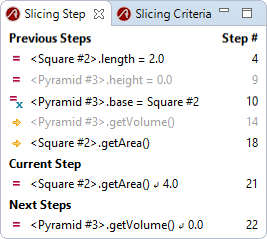
\includegraphics[width=0.40\linewidth]{img/slice1.png}
	\caption{The Slice Navigator shows context for the current debug step. Steps directly related to the current step are listed in black, steps with overarching dependencies in gray. Small icons indicate how the steps are related.}
	\label{fig:slice1}
\end{figure}

To produce a slice, dynamic or static, slicing tools have to build up deep knowledge of a program's internal workings.
In the end, only a binary mapping about which instruction to include or exclude from the program is returned, and most of the slicer's internal knowledge is discarded.
Hence, the initial motivation for the Slice Navigator was to make better use of a slicer's internal data.
However, since the size of all dependency graphs is typically too vast to be visualized at once, we propose to use that data to guide developers while they debug the slice.

The first purpose of the Slice Navigator is to aid the developer's short-term memory.
It provides a quick overview over previous and upcoming events, and how they relate to the current instruction.
\Cref{fig:slice1} shows a screenshot of the slice navigator with the execution of the example test-case halted on the ´return´ instruction of ´getArea()´ in \linerefn{lst:example}{7}.

A step, or event, is any instruction that has a side effect on the program state.
"Previous Steps" lists all past events that the current or any future events depend on.
Likewise, "Next Steps" shows all events that depend on the current or a previous event.

If a step is shown in black, it has a direct dependency link to the current step.
Steps shown in gray have dependencies that go beyond the current step.
I.e., gray "previous steps" have dependency links to "next steps", and vice versa.

Simply by looking at the previous and next steps, the developer can understand at a glace how the current instruction fits into the greater scheme.
This is particularly useful if the current instruction was reached via a breakpoint, in which case it is not always obvious at which point in time it was hit.

To obtain this kind of information with a regular debugger, developers need to analyze the execution stack and maybe even inspect lower stack frames.
But even then it is not always obvious which part of the program state that is still reachable is actually used again.
Unlike a typical debugger's variable view, the Slice Navigator only shows relevant variables, and also shows relevant object fields on the first level.

Further, the Slice Navigator shows details about the dependency graph that was used to compute the current slice.
Small icons indicate how the events of the slice are related.
The meaning of these symbols will be explained in the next subsection.

The second purpose is to serve as a convenient interface to the debugger.
Debugging with the Slice Navigator is simple:
To investigate the origin of a value, developers can simply click on it to move the execution to that point in time.
This way, the slice navigator allows to efficiently follow infection chains of erroneous state.
Likewise, it is easy to follow up on the impact of an instruction by navigating to its future dependencies.

However, using the Slice Navigator developers can not only control the debugger, they can also adjust the slicing criteria.

\section{Incremental Configurable Slicing Algorithm}

\tmpStart
In principle, the Slice Navigator can run on top of any slicing algorithm.
However, for most effectiveness, the algorithm should satisfy three criteria:
First, it should be able to quickly produce useful intermediate results to avoid interrupting developers in their work.
Second, if it distinguishes between different types of dependencies, the differences between those types should be easily understandable for developers.
This way, additional helpful information can be communicated to the user and better customization of the slice is possible.
Finally, it should support incrementally changing the slicing criteria.
The algorithm we use in our prototype is specifically engineered to meet these criteria.

%The algorithm we use in our prototype is based on previous work~\cite{treffer_dynamic_2014} and specifically engineered to meet these criteria.
%When building the dependency graph between instructions, the algorithm distinguishes between three types of dependencies.
%
%\emph{Value dependencies} occur when the the value of an instruction is derived from another instruction's value.
%In the slice navigator, they are represented with a red equality sign.
%
%Instructions that determine if another instruction can be reached are \emph{reachability dependencies}, indicated by a yellow arrow.
%Typically, these are method invocations and instruction in conditional statements.
%
%Sometimes, a value depends on only one of multiple candidate values. 
%A \emph{control dependency} determines which of these candidates is used.
%More formally, control dependencies are reachability dependencies of value candidates that are not also reachability dependencies of all other candidates.
%In the navigator, they are indicated by a blue~"X".
%
%Developers can now combine these different dependency types to adjust the slice for specific purposes.
%Clicking on an event's dependency symbol brings up a dialog that allows to choose which dependencies of that event to include.
%This way developers can, for instance, put a focus on how a value was computed or how an instruction was reached.
%It is also possible to remove all dependencies of an event, for instance if it is known to be correct and its history is not of interest, thereby moving the focus of the slice to less well-understood parts of the program.


Typically, static and dynamic slicing algorithms focus on finding statements belonging to a slice.
However, in many cases statements are executed multiple times in a single program run and not all executions are relevant for the slice.
Therefore, our algorithm focuses on state-changing events, i.e., actual executions of statements, instead of the statements themselves.

On the highest level, our algorithm to compute a dynamic slice works as follows:
The output of the algorithm will be a sorted set of events.
The target event, i.e., the event for which the slice was requested, is added to both the result set and a queue of unprocessed events.
Then, until the queue is empty, an event is polled and its dependency events are determined as follows:

%Firstly, the event is mapped to a unit of a \verb+SootMethod+.
Firstly, the event is mapped to a statement in the code.
Secondly, Soot is used to obtain a static dependency graph for that method (the graph is cached for reuse).
Thirdly, the statement is looked-up in the graph and candidate dependency statements are mapped back to events.

Each dependency event that is not yet part of the result set is added to both the result and the queue.
Finally, the result set is returned.

\begin{figure*}[t]
\centering
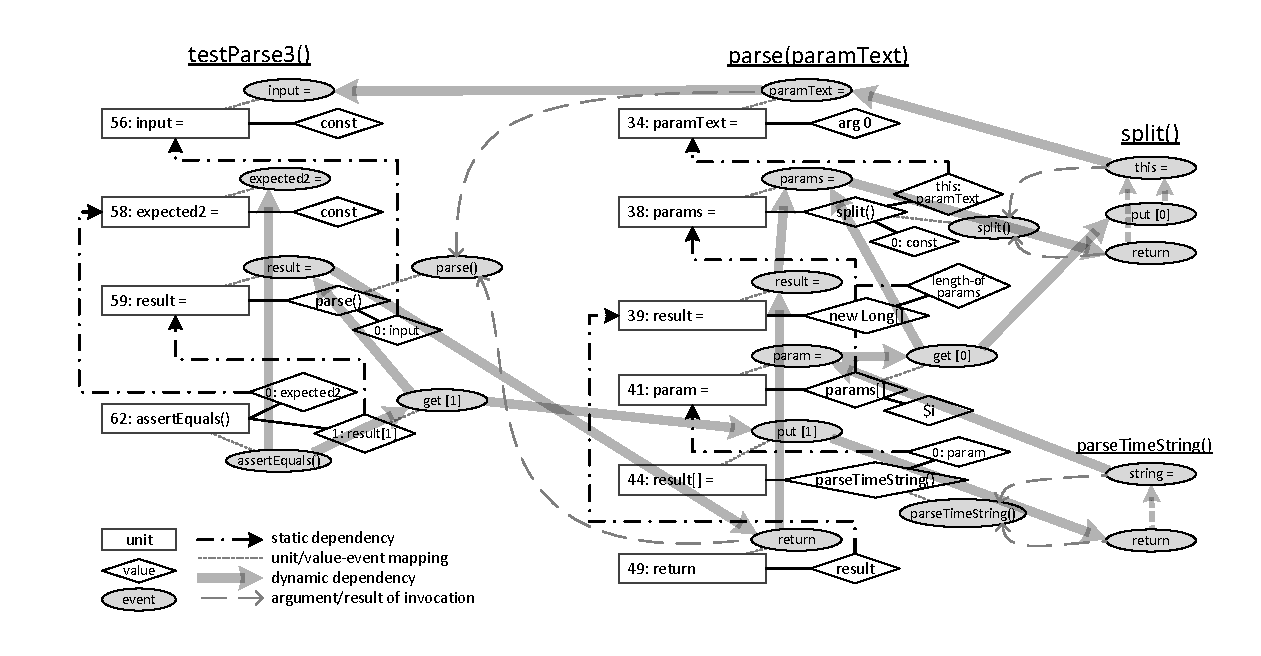
\includegraphics[width=.90\linewidth, clip, trim=12mm 7mm 8mm 7mm]{img/graph}
\caption{A dynamic dependency graph of trace events, on top of static dependency graphs derived with Soot. For brevity, not all Soot units are shown, the boxing of long values has been omitted, and ``split'' and ``parseTimeString'' are summarized.}
\label{fig:graph}
\end{figure*}

\subsection{Computing the Dependency Graph}

In the dependency graph, three types of dependencies are distinguished: value, reachability, and control dependencies.

Value dependencies are the most common, they occur whenever a value is derived from another value.
For instance, the value of \verb+params+ in \linerefn{lst:parse}{38} of \verb+parse()+ depends on the result of \verb+split()+ (cf. \autoref{lst:parse}).

Reachability dependencies refer to expressions whose values determine whether the statement could be reached.
For the assignment in \linerefn{lst:parse}{44} one reachability dependency is the result of \verb+length()+ in \linerefn{lst:parse}{41}.

Control dependencies occur when a statement can have multiple candidate dependencies.
In the statement \lstinline{var = foo() ? bar() : baz()}, the value of \verb+var+ depends on either \verb+bar()+ or \verb+baz()+.
Even though \verb+foo()+ does not directly affect the value, it determines which of the two options is used; thus, it is a control dependency.

In previous work, reachability dependencies are often called ``control dependencies'', while control dependencies as we define them are not considered at all. 
This seems reasonable, as they are only a redundant way to model reachability dependencies.
We introduced this distinction after a small survey between colleagues revealed that some developers found it counter-intuitive to find statements in a slice that do not directly affect the resulting values, while others wanted to have those statements included, as they could help to understand how a certain line in the code could have been reached.
Distinguishing between these two types of control flow dependencies allows us to create a slice specifically for the user's needs.

The algorithm to build the dependency graph was implemented in Soot, using a \verb+ForwardFlowAnalysis+.
In Soot, a method is represented by three-address-code instructions, called ``units''.
A flow analysis ``flows through'' (i.e., visits) every unit in a method and allows to pass state in a ``flow set'' from one instruction to the next.
If a unit has more than one following unit, (e.g., it is a conditional jump) a copy of the flow set is passed to each.
If multiple flow sets appear as input to a flow step, they are merged into one first and only the result of the merge is passed on.
The flow and merge steps of our implementation are shown as pseudocode in \autoref{lst:visit}.


\begin{lstlisting}[firstnumber=1,float,caption={Our dependency algorithm in pseudocode.},stepnumber=5,label=lst:visit,gobble=0,language=algorithm,tabsize=2]
function visit(DataDependencyFlow in, Unit unit, DataDependencyFlow out)
	in.copyTo(out)
	DataDependency dependency = getDependencies(unit.getUseBoxes(), out)
	if unit is_a IfStmt or unit is_a LookUpSwitchStmt then
		out.reachabilityDependencies << dependency
	else
		out.valueDependency = dependency
		if unit is_a DefinitionStmt then
			left = d.getLeftOp()
			indexAssignment(left, unit)
			if left is_a JimpleLocal then
				out.variableChanged(left.name, unit)
		else if unit is_a ReturnStmt or unit is_a ReturnVoidStmt then
			indexReturn(unit)
		else if unit is_a ThrowStmt then
			indexThrow(unit)

function getDependencies(List values, DataDependencyFlow out)
	allDependencies = []
	for v in values do
		allDependencies << getDependency(v, out)
	return DataDependency.all(allDependencies)

function getDependency(Value v, DataDependencyFlow out)
	if v is_a JimpleLocal then
		return out.getVariable(v.name)
	else if v is_a InvokeExpr then
		d = DataDependency.Invoke(v.method,
			getDependency(v.instance, out),
			getDependencies(v.arguments, out))
		indexInvocation(d)
		return d
	else if v is_a InstanceFieldRef
		return DataDependency.field(v.name,
			getDependency(v.instance))
	else 
		...

function merge(DataDependencyFlow in1, DataDependencyFlow in2, DataDependencyFlow out)
	in1.copyTo(out)
	controlDependency = ' delta of in2.reachabilityDependencies and out.reachabilityDependencies, or the last element of both
	out.reachabilityDependencies.remove( controlDependency)
	for var in in2.variables do
		outValue = out.getVariable(var.name)
		if var.value != outValue then
      mergedValue = DataDependency.choice(
            controlDependency, 
            var.value, outValue)
			out.setVariable(var.name, mergedValue)
\end{lstlisting}


A customized FlowSet was implemented that, additionally to existing operations, maintains a stack of reachability dependencies and tracks the current value for each variable, i.e., mostly the unit where it was set last.

For each unit that is visited, its dependencies are determined from its ``use boxes'', the values accessed by the unit.
If the unit represents an if- or switch-statement, the dependencies are pushed to the outflow as reachability dependencies.
Otherwise, they are value dependencies of the unit.
If the unit assigns a variable, it is also registered to be the last unit that changed that variable.

Furthermore, each unit is indexed:
A unique key is created from the unit's line number and its type. 
If the unit assigns a variable or field, the respective name is also part of the key.
The index is stored as a map and will be used later to find the unit for a given event.

To obtain a list of dependencies from a list of value boxes, each value is examined independently.
If it refers to a variable, the value of the variable currently stored in the flow is used.
Field and array accesses are not investigated any deeper, and simply noted along with the current line number.
Method invocations are also treated as opaque, and no dependency between the invocation result and its arguments is created.
Instead, the dependencies for each argument are determined separately and directly added to the index, with a unique key being created for each argument.
It is expected that the subsequent analysis of the invoked method reveals, if necessary, how an invocation's result depends on its arguments.

In the merge step of the analysis, the first incoming flow set is copied to the destination set, which is then merged with the second incoming set.

To merge two flow sets, first their reachability dependency stacks have to be aligned.
If the stacks contain different elements, only dependencies from both stacks are kept.
If both stacks are identical, for instance when merging the then- and else-branch of an if-statement, the topmost element of the stack is removed.

Then, all variables that have different values have to be merged.
Instead of a definite unit, the new value is a choice of the two previous values, indicating that at in the dynamic slice only one of the options will actually apply.
Furthermore, the reachability dependencies that have been removed during the merge are added here as control dependencies.

For reference, \autoref{fig:graph} shows parts of the static dependency graphs from both methods listed above.
The dynamic dependency graph has been included in the figure as well, to visualize the relation between the static and dynamic elements.

\subsection{Mapping Events and Units}

Before the dependencies of an event can be found, it has to be mapped to a Soot unit.
The event provides class and method name, line number, and byte-code index as locational information.

Alas, we were not able to find the corresponding unit based on the byte-code index.
Instead, the event type and line number are used to look-up units in the index that was created during the flow analysis.
For an averagely structured Java program, ambiguities occur only rarely.
As shown on the bottom left of \autoref{fig:graph}, in our example the slice would begin with the \verb+assertEquals+ invocation, which can be mapped to the invocation unit in \linerefn{lst:test}{62}.

Once the unit has been identified, its dependencies are looked-up and converted back to events.
Reachability dependencies are included only if they have been explicitly requested.
%How events are looked-up depends on the type of the dependencies.
The dependency value's line number and the current event's step number are used to identify the most recent matching event.
However, the strategy of the look-up also depends on the type of the dependency value.

If the dependency is an assignment statement of a variable, the last variable change event in that line is looked-up.
For instance, the dependency between the \verb+assertEquals+ invocation and the \verb+expected2+ assignment is created this way.
If it is a choice of multiple variable assignments, each assignment is looked-up and, if more than one is found, only the most recent will be used.

For field and array value dependencies, first the according get-event is looked-up.
Then, the last set-event before the get is found.
For instance, this allows us to create a dynamic dependency between \verb+assertEquals+ and the array assignment in the second iteration of \verb+parse+ (shown on the right-hand side of \autoref{fig:graph} as the ``put'' event linked to the assignment in \linerefn{lst:parse}{44}).
Finding the get as an intermediate step is necessary to avoid situations where the field has been changed between access and usage, e.g., as in \verb/int id = counter++/.

If the value stems from an argument, first the calling method is determined from the trace data. 
Then, the argument is looked up in the index of the dependency graph of the calling method.
Finally, the dependencies retrieved this way are resolved recursively.
To get the result of an invocation, the method call event is looked-up and its respective return event is found.
As \autoref{fig:graph} shows, the invocation of \verb+parse+ is not part of the dynamic dependency graph because it is an event without side effects.
However, it serves as the link to create dependencies between events of the two methods.

All events that are found this way are added to the slice.
If an event was found via a unit, this information is retained and reused when computing the dependencies for that event.

The final list of events is the used by the debugger to visualize the program flow and to skip unrelated events during stepping.

\begin{figure}
	\centering
		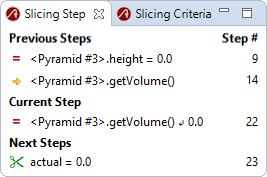
\includegraphics[width=0.40\linewidth]{img/slice2.png}
	\caption{The program halted at \linerefn{lst:example}{21}, after \lstinline{getArea()} was removed from the slice.}
	\label{fig:slice2}
\end{figure}

Whenever a slicing criterion is modified, the slice is updated instantly, without locking the user interface or resetting the current debug session.
In our examples, developers might choose to exclude the result of ´getArea()´ from the slice as it is correct.
As shown in \cref{fig:slice2}, with the computation of the area removed from the slice it is now much easier to see that the wrong result of ´getVolume()´ was caused by a wrong value in ´height´.

As mentioned before, instructions and states not belonging to the slice are still shown in the IDE, mostly to serve as an orientation help, to provide context to the current operations.
However, it might also happen that a value or instruction outside of the slice catches a developers attention.
In this case, they can choose to add it as another slicing criterion and the slice is immediately expanded.
Again, this happens without interrupting the developer's work.

After some preliminary user testing, we added two shortcuts for frequently used operations.
Right-clicking an entry immediately removes it entirely from the slice, while double-clicking an entry sets it as a slicing criterion and removes all previous criteria.
\tmpEnd

\section{The Slice Navigator}

\section{Performance Considerations}
\label{sec:eval}

\section{User Study}

\tmpStart
We evaluated our approach in two ways.
First, we measured the run-time of the slicing component for various operations on a real-world project and found it to be fast enough to be usable in practice.
Second, we let developers locate bugs using different tools and interviewed them about their experience.
The experiment confirmed the usefulness of the Slice Navigator and provided suggestions for further improvements of our tool.

\subsection{Performance Considerations}

One of the main advantages of the Slice Navigator is that it integrates into the debugging workflow.
As such, it is crucial that results are produced in a timely manner, as a waiting time of even a few seconds may interrupt developers in their flow.

To evaluate the performance of our approach on real-world code, we measured the computation of several slices on JUnit tests of an open-source business-process engine\footnote{\url{https://github.com/camunda/camunda-bpm-platform}}.
All tests were run on a 2.0 GHz Intel i7 Processor with 4 cores and and 8 GB RAM, running Windows 8.1.
A MySql database was used to store the trace data.
We repeated every measurement 10 times, all charts show the average values.

\begin{figure}
	\centering
		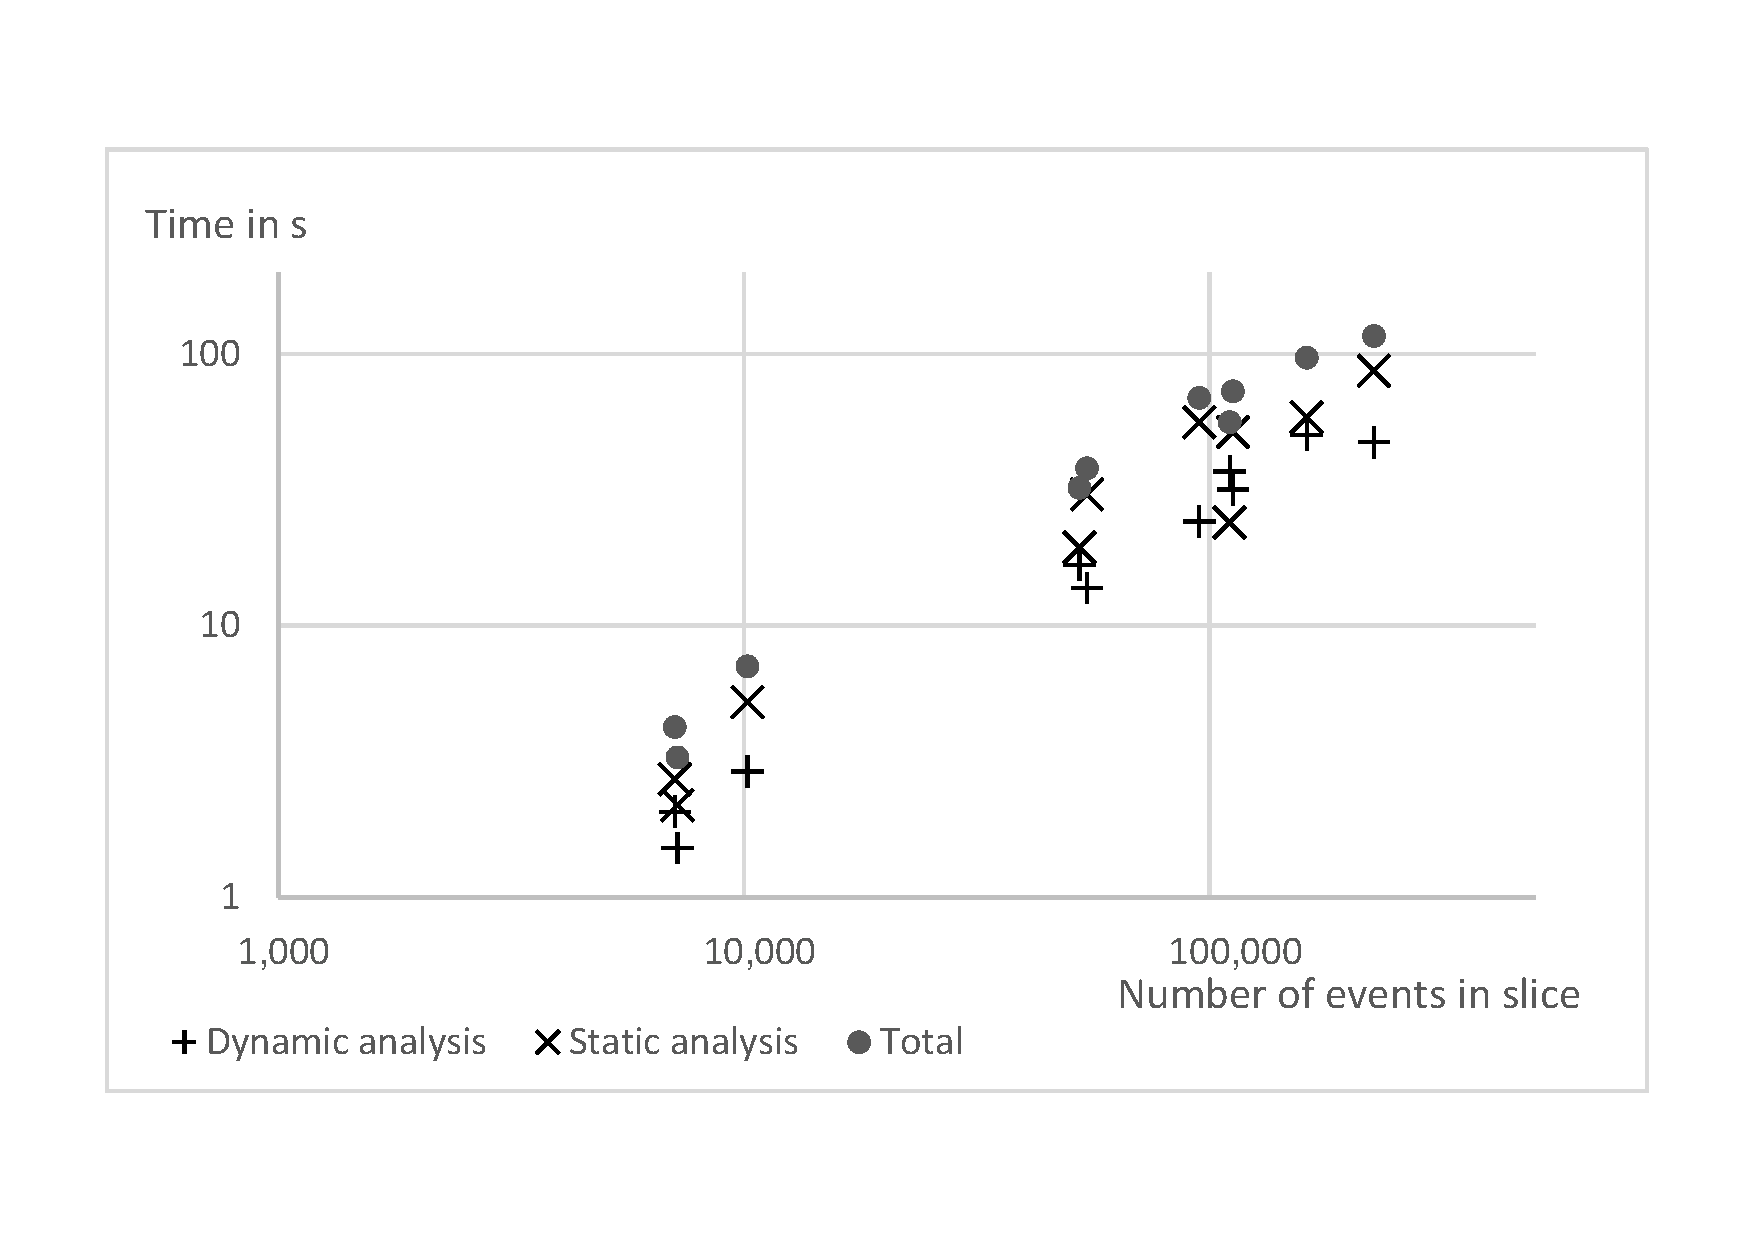
\includegraphics[width=\linewidth, clip, trim={20mm 26mm 20mm 26mm}]{img/chart-initial.pdf}
	\caption{Time for computing the initial slice}
	\label{fig:chartinitial}
\end{figure}

We previously observed that our approach differs from other slicing implementations insofar as that the run-time of the algorithm does not depend on the total length or run-time of the sliced program, but only on the size of the resulting slice~\cite{treffer_dynamic_2014}.
Our current measurements confirm that slicing time is linear to the result size.

\Cref{fig:chartinitial} shows the time for computing the initial slice in seconds, depending on size of the resulting slice.
Times are given in total, and divided into static code analysis and the dynamic analysis of the event data.

As can be seen, the static analysis takes slightly more time on average.
It should be noted that the total time is less than the sum of the static and dynamic analysis times, as both can, to some extent, run in parallel.
The chart shows that in our setup the algorithm was able to process approximately 1000 events per second.

\begin{figure}
	\centering
		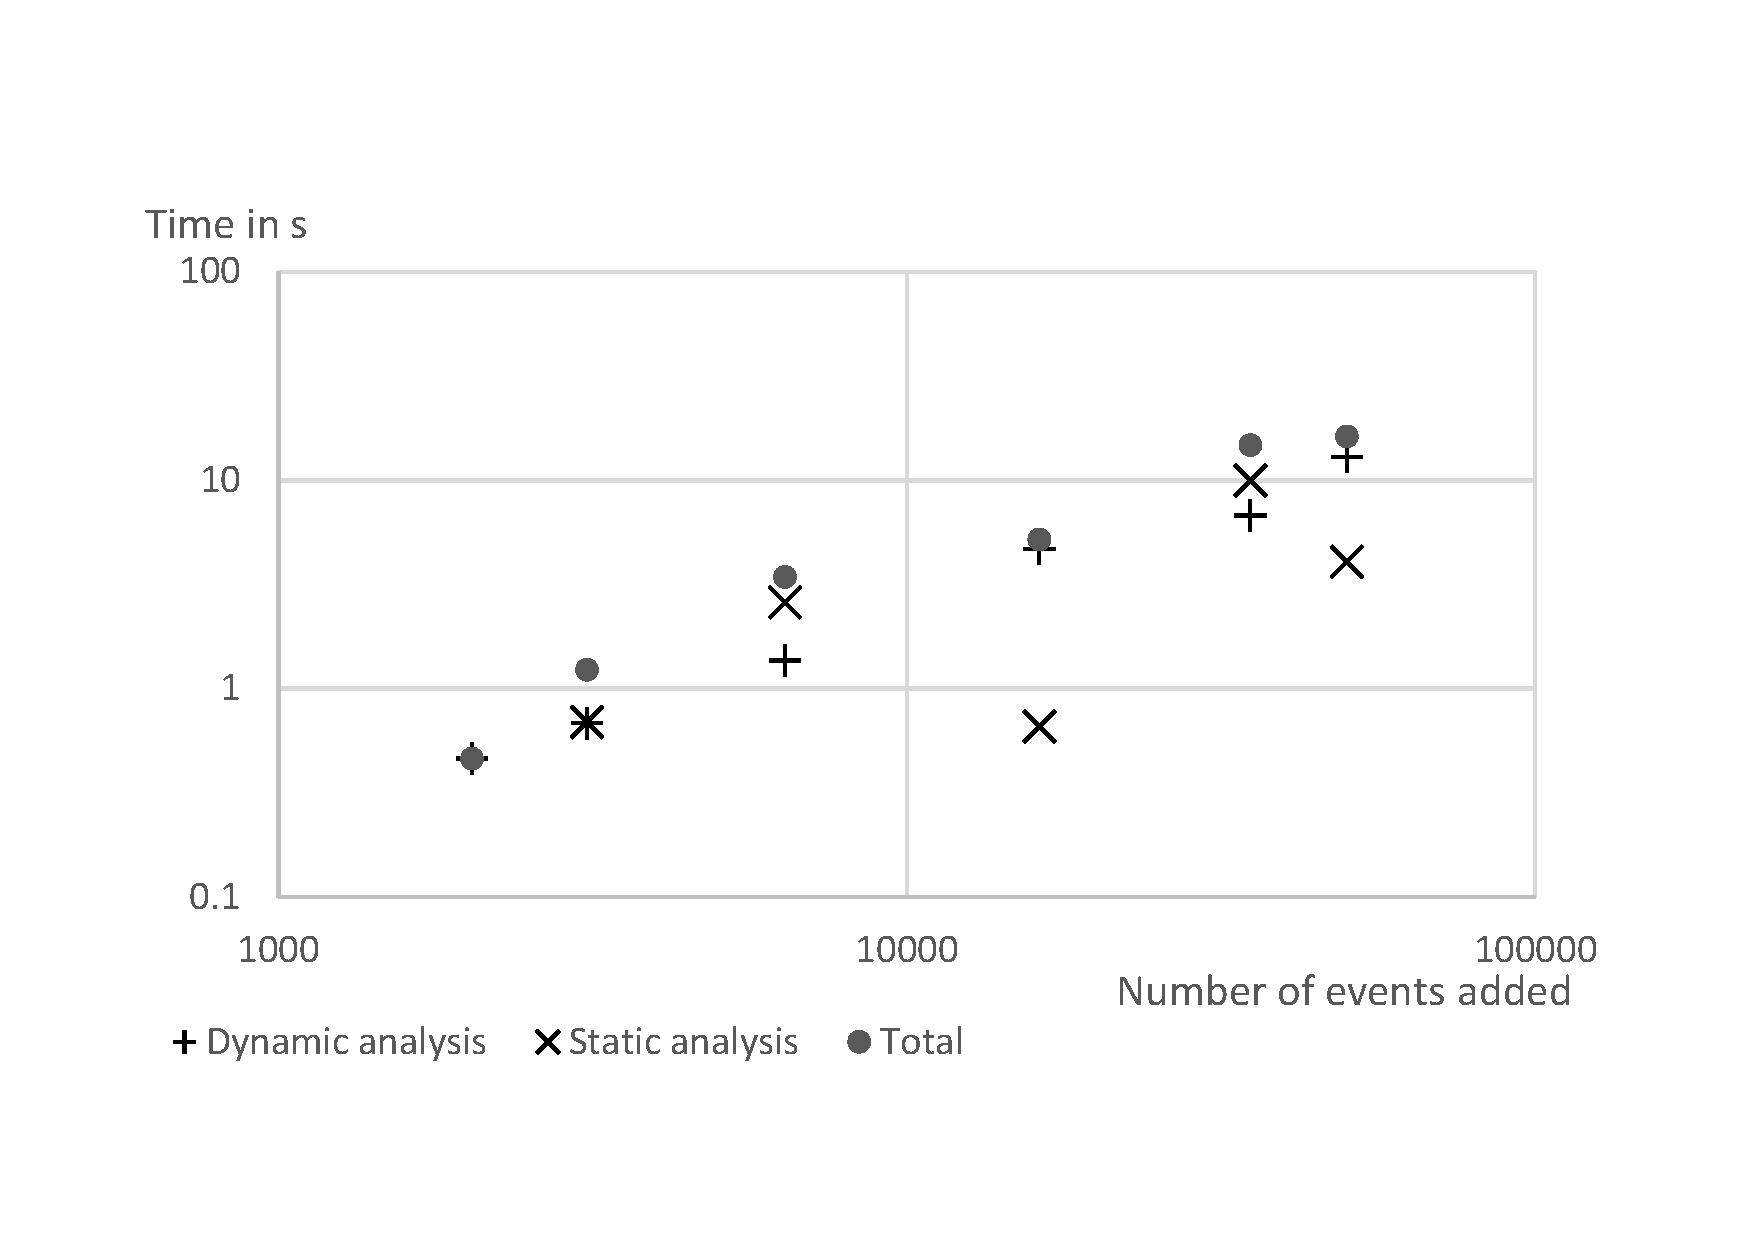
\includegraphics[width=\linewidth, clip, trim={20mm 26mm 20mm 26mm}]{img/chart-add.pdf}
	\caption{Time for adding a slicing criterion}
	\label{fig:chartadd}
\end{figure}

When adding additional elements to the slice, previously computed dependency graphs can be reused.
As \cref{fig:chartadd} shows, the time for dynamic analysis remains constant per event.
The time for static analysis, on the other hand, shows great variation and depends on how much new code was included by the broadened slicing criteria.
In the worst case, expanding the slice takes as long as creating a new slice for only that event.

\begin{figure}
	\centering
		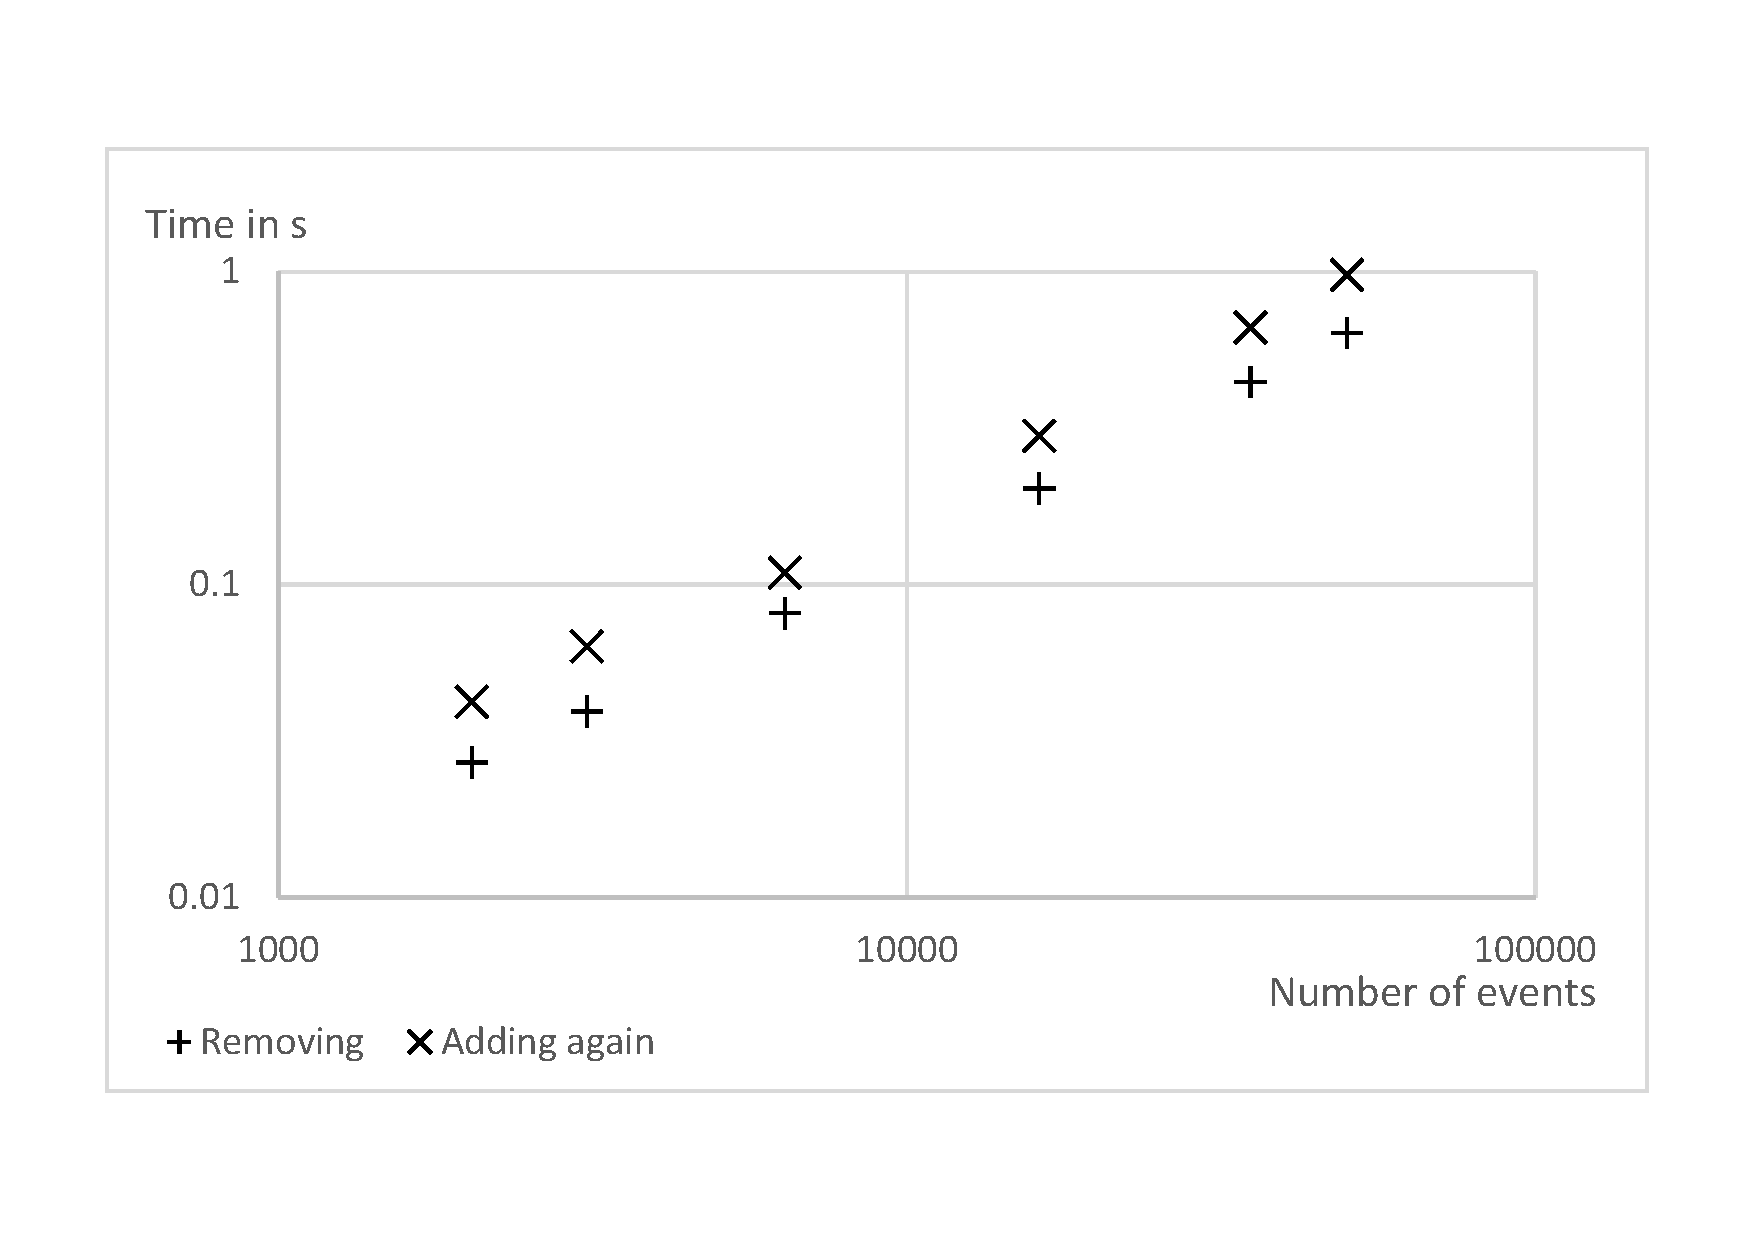
\includegraphics[width=\linewidth, clip, trim={20mm 26mm 20mm 26mm}]{img/chart-rem.pdf}
	\caption{Time for removing events from the slice}
	\label{fig:chartrem}
\end{figure}

\Cref{fig:chartrem} shows that removing events from the slice by narrowing the slicing criteria is significantly faster, as no actual analysis has to be performed.
Likewise, adding those events again by reverting the slicing criteria change is fast, as previously computed dependency graphs can be reused.

\medskip

From the results in \cref{fig:chartinitial}, it seems as if the slicing algorithm is too slow to be of practical use to a developer.
A single second of execution can produce several hundreds of thousands of events and it is generally not feasible to wait multiple minutes for the slicing to complete.
However, due to parallelization and the way the algorithm works, developers experience a delay of only a few seconds.

As described above, the debugging user interface is updated with an intermediate slicing result twice per second.
The slicing algorithm works its way backwards, beginning at the slicing criteria.
Then, previous events are processed not ordered by their absolute position in the execution, but by their distance in the dependency graph.
As a result, both the near past and long-running overarching method invocations are processed first.

This allows developers to begin debugging the slice almost immediately. 
From this point on, the slicer only needs to be faster than the developer moving backwards, which is generally given.

For interactive changes of slicing criteria, our experiments have shown that the incremental slicing algorithm is fast enough to not interrupt the developers flow.
In particular, the most common operation -- removing events by narrowing the slicing criteria -- completes in less than a second even for large numbers of events.
From this we conclude that our debugging approach, based on the Slice Navigator and on iterative slice refinements, is generally feasible.

\subsection{User Study}

To gather empirical data on the usefulness of our approach, we conducted an experiment where we let developers locate bugs using a regular debugger, the omniscient debugger from our debugging framework, and the Slice Navigator, and compared their experiences.

We used Defects4J, a database of actual bugs from various open-source projects~\cite{just_defects4j_2014}, to find suitable debugging tasks.
For each bug, Defects4J also provides at least one failing test case and the fix.

We chose to conduct the experiment with \emph{Joda Time}\footnote{\url{http://www.joda.org/joda-time/}}, a date and time library for Java, because it has a domain that everyone is already familiar with.
From the Defects4J bug database, we selected Joda Time bugs 10, 19, and 27.

The bugs were selected because they can be fixed with a small change at a single code location and require not much knowledge about the more technical details of Joda Time.
Furthermore, all bugs are from different parts of the project, so that in our experiment the order of the bugs will have no impact on the developers' familiarity with the code.
Finally, each bug is caused by a different kind of defect:
the first bug is caused by a wrong hard-coded constant value;
the second bug is caused by wrongly skipped code, i.e., a too restrictive \textit{if}-condition;
while the third bug is caused by code that should be skipped, i.e., a missing \textit{if} statement.
We expect that the usefulness of each debugging tool varies depending on the nature of the bug.

We recruited nine participants for our experiment:
two full-time software developers with at least 15 years of programming experience, 
four PhD students in computer science with at least 10 years of programming experience,
and three computer science graduate students with at least 5 years of programming experience who also worked as programmers in a part-time job for at least one year.
Ages of participants ranged between 25 and 36; one PhD student was female, all other participants were male.
No participant had previous experience with Joda Time, although 5 participants were aware of its existence.

Every participant was tasked to find the location of each bug by debugging the failing test case with one of the tools.
With the Slice Navigator, we specifically asked the participants not to use the other features of the omniscient debugger and reminded them during the task if necessary.
In the end, every participant had used each tool and every bug was examined with each tool three times.

For each debugging task, the procedure was as follows:
First, the participant was shown a passing test case similar to the test case they would later have to debug.
We explained the purpose of the test and started the debugging tool to be used.
Then, we let the participant debug the test case, while we explained both the code and the tool.
When the participant had no more questions, we presented the failing test case and explained the semantics of the failure.
Then we asked the participant to locate the bug using the respective tool and started the timer.
During the debug session, we provided tool support when needed.
If a bug could not be located within 20 minutes, we aborted the task to advance the experiment.

\subsubsection{Comparison of Tool Usage}

\begin{figure}
	\centering
		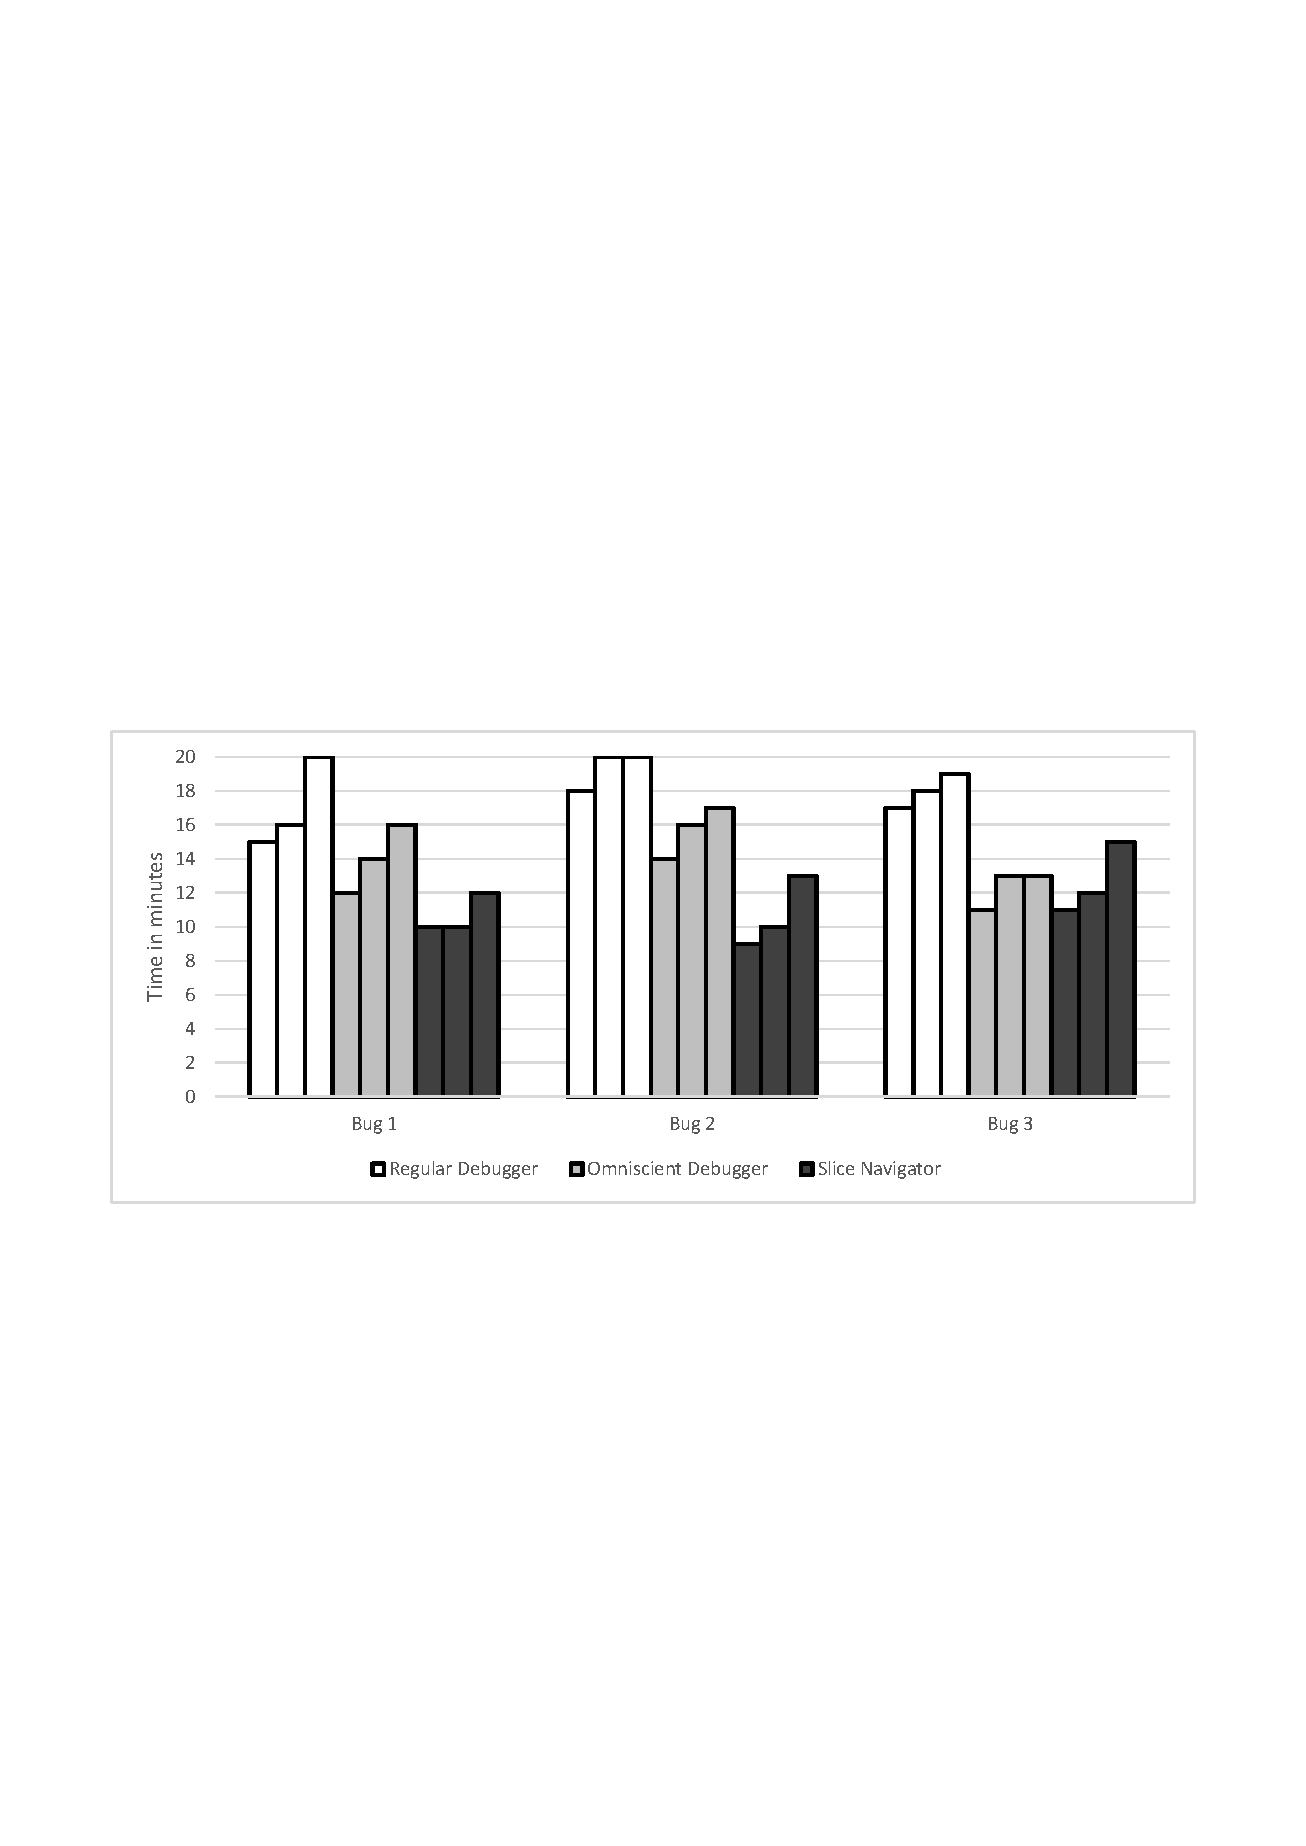
\includegraphics[width=\linewidth, clip, trim={20mm 110mm 19mm 125mm}]{img/chart-times.pdf}
	\caption{Time for solving each debugging task.}
	\label{fig:charttimes}
\end{figure}

\Cref{fig:charttimes} shows the time taken for each debugging task.
The data suggests that the Slice Navigator can make debugging more efficient in many cases.
Furthermore, we observed changes in developer behavior when using different tools.

With the Eclipse debugger, three participants made heavy use of the "inspect" feature, which evaluates any expression from the source without further executing the program.
In particular, when contemplating whether to step into or over a method invocation, these participants used "inspect" to preview the invocation result.
This shows a general need for moving more freely in time.
The three participants who used "inspect" had to restart the debugger 2, 3, and 4 times, respectively, while the other participants restarted between 6 and 12 times, and accidentally stepped over a method between 2 and 5 times per task.

Furthermore, 5 participants stopped using the debugger entirely for more than a minute, and spent 2 to 7 minutes with pure code reading and mentally simulating the program.

The omniscient debugger was particularly effective for the third bug, where all three participants found that a valid field value was overridden by inspecting the object history.
This allowed them to form a good theory about the nature of the bug very early.
However, the method containing the bug was invoked at two different points in time and each time also called itself recursively.
The bug occurred only in one of the four executions.
With the omniscient debugger, it took developers a while to notice and distinguish the different invocations as they jumped through time.
Overall, with the omniscient debugger all 9 developers felt \emph{lost in time} between 2 and 9 times (average 5.4($\pm1.3$)) per debug session.

Finally, while all developers used the omniscient debugger to step back and forth repeatedly to understand the side effects of a piece of code, 7 developers spend most of their time following the infection chain backwards, while 2 developers mostly debugged forwards in time, like they would with a regular debugger.

With the Slice Navigator, all developers followed the infection chain backwards.
Compared to using only the omniscient debugger, developers where able to reach the end of the infection chain faster, felt lost in time similarly often (on average 5.4($\pm2.0$) times), but took longer to recover from being lost as they had spent less time understanding the code.
However, with the Slice Navigator, developers spent only 0.9($\pm0.6$) minutes per task reading code entirely unrelated to the bug, compared to 4.3($\pm1.8$) minutes with the other tools.

\subsubsection{Developer Experiences}

After the experiments, we asked the participants how they experienced working with the different tools.

All participants reported that they found it very helpful to be able to go back and forth in time with the omniscient debugger and felt that they could use it more effectively with more experience, as being used to regular debuggers limited their way of thinking.
7 participants said they were at times overwhelmed with the amount of available options and would probably use more of the more advanced features with more experience.
Furthermore, 6 participants expected they would end up lost-in-time less often with code that they are more familiar with.

For the Slice Navigator, we received similar feedback about moving freely trough time.
Furthermore, all participants liked how the Slice Navigator helped to identify relevant program state.
5 participants perceived this as an improvement in particular to the omniscient debugger, as it was less overwhelming.

However, 4 participants found the overarching dependencies shown in gray to be unnecessary and distracting and emphasized the usefulness of being able to double-click an entry to improve the focus of the slice.
On the other hand, 2 participants said they generally liked the idea of seeing relevant state and would probably find it more useful with code they were more familiar with.

Every participant wrongly clicked or double-clicked an entry at least once and was then unable to recover quickly from the mistake.
Thus, an undo-button was requested by all participants.

Finally, 3 participants reported that while the information provided by the Slice Navigator was very useful, they found it distracted from the actual code.
They liked that with a regular debugger they would rarely have to look away from the code and wished for the slicing context to be visualized within the IDE's code editor.

\subsubsection{Threats to Validity}

The main concern to our study is the small number of participants, which does not allow to generalize the results.
All results could be the product of statistical anomalies.
Furthermore, our participant group was very heterogeneous with respect to programming experience,
although we observed no difference in tool usage or skill level between the different groups.
This effect has been observed in previous studies~\cite{host_using_2000, salman_are_2015}.
Nevertheless, some limitations apply~\cite{mcmeekin_significance_2009}.

Likewise, we only considered three bugs from one library.
Although they are real bugs, they all could be tracked down to one location.
For more complex bugs, or bugs in different types of applications, such as web applications, the usefulness of each tool can differ.
A follow-up study should observe programmers using the tools in practice.

Furthermore, all participants were unfamiliar with the code they had to work with.
We accounted for this in two ways.
First, to achieve the same level of initial knowledge for each task, all bugs were chosen from different parts of the library.
Second, each participant received an introduction to the code to be debugged.
Nevertheless, many participants argued they would have used the tools differently with familiar code.

\tmpEnd